\documentclass[12pt, twoside]{article} 

\usepackage[a4paper]{geometry}
\usepackage[english]{babel}
\usepackage[utf8]{inputenc}
\usepackage[T1]{fontenc}
\usepackage[scaled]{helvet}
\renewcommand\familydefault{\sfdefault}
\usepackage{enumitem}
\usepackage{amssymb}
\usepackage{url}
\usepackage{pdfpages}
\usepackage{fancyhdr}
\usepackage{sectsty}
\usepackage{hyperref}

% Bibliography
\usepackage[backend=biber]{biblatex}
\usepackage{csquotes}
\addbibresource{references.bib}

% Section font sizes
\sectionfont{\fontsize{22}{26}\selectfont}
\subsectionfont{\fontsize{20}{24}\selectfont}
\subsubsectionfont{\fontsize{18}{22}\selectfont}

% Increase paragraph spacing
\setlength{\parskip}{1em}
\setlength{\parindent}{0pt}

% Set margins
\setlength{\hoffset}{-1.1in}
\setlength{\voffset}{-1in}
\setlength{\oddsidemargin}{2cm}
\setlength{\evensidemargin}{2cm}
\setlength{\topmargin}{0.7cm}
\setlength{\headheight}{1.2cm}
\setlength{\headsep}{0.4cm}
\setlength{\textheight}{25.7cm}
\setlength{\textwidth}{17.5cm}
\setlength{\footskip}{1.0cm}
\setlength{\columnsep}{0.5cm}

% Hyperref setup
\hypersetup{
    colorlinks=true,
    linkcolor=blue,
    urlcolor=blue,
    citecolor=blue,
}

% Array rule width and row spacing
\setlength{\arrayrulewidth}{0.5mm}
\renewcommand{\arraystretch}{1.5}

% Fancyhdr setup
\pagestyle{fancy}
\fancyhf{}
\fancyhead[LE,RO]{Requirements Specification}
\fancyhead[RE,LO]{\textsc{Motion Recovery}}
\fancyfoot[LE,LO]{\leftmark}
\fancyfoot[LE,RO]{\thepage}
\renewcommand{\headrulewidth}{1pt} % Header rule thickness
\renewcommand{\footrulewidth}{1pt} % Footer rule thickness
\setlength{\headheight}{15pt}
\setlength{\footskip}{30pt}
\setlength{\headsep}{30pt}

\begin{document}
    % title page
    \begin{titlepage}
    \setlength{\topmargin}{4cm} % Set a larger top margin for the title page
    \begin{center}
        % Title and Subtitle
        \vfill 
        \begin{minipage}{0.8\textwidth}
            \centering
            {\Huge \textbf{\uppercase{Motion Recovery}}}\\ % Main Title
            \vspace{4mm}
            {\small \textcolor{gray}{\hfill Cahier des charges suivant le template~\cite{volere20} Volere (v.20)}}
        \end{minipage}
        
        % Logo
        \vspace{15mm}
        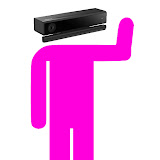
\includegraphics[height=6cm]{images/motion-recovery-logo.jpeg} % Logo
        \vspace{30mm}
        
        % Authors and Date
        \begin{minipage}{0.7\textwidth}
            \centering
            \textsc{LESCEUX Antonin}\\
            \vspace{3mm}
            \textsc{LONGFILS Gerry}\\
            \vspace{3mm}
            \textsc{VERVLOESSEM Lucas}\\
            \vspace{3mm}
            \textsc{SCHWEITZER Kevin}\\
            \vspace{10mm}
            December 2024
        \end{minipage}
        \vfill
    \end{center}
\end{titlepage}

    % table of contents
    \tableofcontents

    %% content
    % section 1 : purpose
    \section{The purpose of the project}
\subsection{The user business or background of the project effort}
\subsection{Goals of the project}

    % section 2 : stakeholders
    \section{Stakeholders}
\subsection{The Client}
\subsection{The Customer}
\subsection{Other Stakeholders}
\subsection{The Hands-On Users of the Product}
\subsection{Personas}
\subsection{Priorities Assigned to Users}
\subsection{User Participation}
\subsection{Maintenance Users and Service Technicians}


    % section 3 : constraints
    \addtocontents{toc}{\protect\newpage}
\section{Constraints}
\subsection{Solution Constraints}
% Definition of a minimalistic box style with rounded corners for the solution constraints
\tcbset{
    minimalcard/.style={
        colback=white,       
        colframe=black,     
        boxrule=0.4mm,      
        arc=4mm,             
        width=\textwidth,   
        outer arc=1mm,       
        boxsep=4pt,          
        left=6pt,            
        right=6pt,           
        top=6pt,             
        bottom=6pt           
    }
}
% Box1
\begin{tcolorbox}[minimalcard]
    \raggedright\textbf{Description}: \vspace{6pt}\\
    The product shall use a Microsoft Kinect to monitor the user's movements during reproduction of exercises. The use of a kinect is an abitrary decision based on the fact that it has proven to be quite successful at using joint monitoring to analyse gesture with precision. The kinect will be provided for the therapist and he will distribute them further to interested patients.\\
    \vspace{6pt}
    \textbf{Rationale}: \vspace{6pt}\\
    A monitoring device capable of analysing movements with a minimum of precision is required for Motion Recovery. Patients and therapists shouldn't directly have to pay a supplement for the cost of such a device.\\
    \vspace{6pt}
    \textbf{Fit Criterion}: \vspace{6pt}\\
    Users have access to the kinect system after integration of Motion Recovery into their physical therapy plan. The acquirement, transportation and installation of the kinect should be simple and successful without advanced technical knowledge.  
\end{tcolorbox}
% Box2
\begin{tcolorbox}[minimalcard]
    \raggedright\textbf{Description}: \vspace{6pt}\\
    Motion Recovery will handle sensitive information in regards to user activities during their recovery. Personal information will also be provided to Motion Recovery. Medical data has to be handled with care and securely. Furthermore, data overall will be handled with respect of GDPR guidelines.\\
    \vspace{6pt}
    \textbf{Rationale}:\\ \vspace{6pt}
    Ensuring the security and privacy of user data is essential to maintain trust between patients, therapists, and the system. Non-compliance with GDPR and other regulations could result in legal and financial consequences, as well as harm the reputation of the system. Proper handling of sensitive information minimizes the risk of unauthorized access, data breaches, or misuse.\\
    \vspace{6pt}
    \textbf{Fit Criterion}:\\ \vspace{6pt}
    All sensitive data is encrypted both in transit and at rest using industry-standard protocols. The system includes user consent mechanisms and a privacy policy in compliance with GDPR. Access to personal and medical data is restricted based on user roles, and audit logs track all access and modifications to such data.
\end{tcolorbox}
\vfill
\hfill
% Box3
\begin{tcolorbox}[minimalcard]
    \raggedright\textbf{Description}: \vspace{6pt}\\
    The Motion Recovery system must include a reporting feature for therapists to track and analyze patient progress. The reports should provide visual and textual feedback on performance metrics such as range of motion, frequency of exercises, and adherence to the prescribed therapy plan.\\
    \vspace{6pt}
    \textbf{Rationale}: \vspace{6pt}\\
    Tracking progress is crucial for therapists to assess recovery, adjust therapy plans, and provide constructive feedback to patients. Clear and accessible reporting ensures therapists can effectively manage multiple patients.\\
    \vspace{6pt}
    \textbf{Fit Criterion}: \vspace{6pt}\\
    The system generates reports that include graphical representations of performance metrics. Therapists can access and download patient reports within a maximum of three clicks. Reports must cover at least a week of activity and allow customization of the metrics displayed.
\end{tcolorbox}

% Box4
\begin{tcolorbox}[minimalcard]
    \raggedright\textbf{Description}: \vspace{6pt}\\
    Motion Recovery will include a personalized exercise library. This library should be customizable by therapists to adapt to individual patient needs and include video instructions, difficulty levels, and alternative exercise options.\\
    \vspace{6pt}
    \textbf{Rationale}: \vspace{6pt}\\
    A flexible, user-specific approach to exercises ensures patients stay motivated and their therapy remains relevant to their progress and limitations.\\
    \vspace{6pt}
    \textbf{Fit Criterion}: \vspace{6pt}\\
    The library supports at least 50 pre-configured exercises with the ability for therapists to add or modify up to 100 custom exercises. Video instructions are accessible in the system for every listed exercise, and therapists can assign and adjust exercises with minimal navigation complexity.
\end{tcolorbox}

% Box5
\begin{tcolorbox}[minimalcard]
    \raggedright\textbf{Description}: \vspace{6pt}\\
    The system must provide real-time feedback on exercise performance, including errors in movement, posture, or timing. Feedback should be displayed in an intuitive, non-intrusive manner, such as visual corrections on a screen or verbal guidance.\\
    \vspace{6pt}
    \textbf{Rationale}: \vspace{6pt}\\
    Real-time feedback helps patients perform exercises correctly, reducing the risk of injury and improving the effectiveness of therapy. Immediate correction is critical for learning proper movements.\\
    \vspace{6pt}
    \textbf{Fit Criterion}: \vspace{6pt}\\
    Feedback latency should not exceed 500 milliseconds. The system provides at least three levels of feedback detail (basic, intermediate, and advanced) and supports both visual and auditory modes of correction.
\end{tcolorbox}
\vfill
\subsection{Implementation Environment of the Current System}
Motion Recovery operates in a distributed environment with Kinect devices for motion tracking, a PC application for exercise logging and live-feedback (active interactions), and a mobile app for viewing progress and receiving notifications (passive interactions). Data is synchronized across all devices via a cloud database, ensuring up-to-date information for both patients and therapists. This environment is designed to be scalable and accessible, using the Kinect for accurate motion tracking at home and the cloud for centralized data storage and management.\par
The web application will have to provide relevant information to the therapist, such as the patient's progress, adherence to the therapy plan and the ability to adjust the therapy plan by updating the database with new exercices or update existing ones. For seamless integration with existing physical therapy tools, Motion Recovery will support data export and import in common formats such as CSV and PDFs.   
\vfill

\subsection{Partner or Collaborative Applications}
\subsection{Off-the-Shelf Software}
\subsection{Anticipated Workplace Environment}
\subsection{Schedule Constraints}
\subsection{Budget Constraints}
\subsection{Enterprise Constraints}

    \printbibliography{}
\end{document}